\documentclass{beamer}
\usepackage{geometry}
\usepackage[english]{babel}
\usepackage[utf8]{inputenc}
\usepackage{amsmath}
\usepackage{amsfonts}
\usepackage{amssymb}
\usepackage{tikz}
\usetikzlibrary{quotes, angles}
\usepackage{graphicx}
\usepackage{multicol}

%\usepackage{pgfplots}
%\pgfplotsset{width=10cm,compat=1.9}
%\usepackage{pgfplotstable}

\setlength{\headheight}{26pt}%doesn't seem to fix warning

\usepackage{fancyhdr}
\pagestyle{fancy}
\fancyhf{}

%\rhead{\small{13 September 2021}}
\lhead{\small{BECA / Dr. Huson / Geometry Unit 7}}

\renewcommand{\headrulewidth}{0pt}

\title{Mathematics Class Slides}
\subtitle{Bronx Early College Academy}
\author{Christopher J. Huson PhD}
\date{16 February 2022}

\begin{document}
\frame{\titlepage}
\section[Outline]{}
\frame{\tableofcontents}

\section{7.13 Similarity - Open Middle intro, 16 February 2022}


\frame
{
  \frametitle{Open Middle problem (fun) \\
  Use digits from 0 to 9. Using a digit no more than once.}
    The first two angle measures are complementary. The second two angles supplementary. (degrees)\\[0.75cm]
      \begin{tikzpicture}
        \draw (0,0) rectangle (1,1);
        \draw (1.25,0) rectangle (2.25,1);
        \draw (3.25,0) rectangle (4.25,1);
        \draw (4.5,0) rectangle (5.5,1);

        \draw (-1.25,-1.5) rectangle (-0.25,-0.5);
        \draw (0,-1.5) rectangle (1,-0.5);
        \draw (1.25,-1.5) rectangle (2.25,-0.5);
        \draw (3.25,-1.5) rectangle (4.25,-0.5);
        \draw (4.5,-1.5) rectangle (5.5,-0.5);
      \end{tikzpicture} \vspace{5cm} 
}

\frame
{
  \frametitle{Do Now:
  Use integers from $1$ to 9, at most once each.}
  Place a digit in each box to create three numbers whose sum is closest to 1000.\\[0.75cm]

 \framebox(15,15){} \framebox(15,15){} \framebox(15,15){} \Large{+}
 \framebox(15,15){} \framebox(15,15){} \framebox(15,15){} \Large{+}
 \framebox(15,15){} \framebox(15,15){} \framebox(15,15){}
}

\frame
{
  \frametitle{Do Now:
  Use integers from $-9$ to 9, at most once each.
  Place a digit in each box to create endpoints for different line segments whose midpoint is $(1, 3)$.}
  
  1. $\overline{AB}$ should have a positive slope, and $\overline{CD}$ should have a negative slope. \\[0.25cm]

  \Large{A(} \framebox(15,15){} , \framebox(15,15){} \Large{)} -- 
  \Large{B(} \framebox(15,15){} , \framebox(15,15){} \Large{)} 

  \Large{C(} \framebox(15,15){} , \framebox(15,15){} \Large{)} -- 
  \Large{D(} \framebox(15,15){} , \framebox(15,15){} \Large{)} \vspace{0.25cm}

  2. Create endpoints for the longest possible line segment $\overline{EF}$ whose midpoint is $(1, 3)$.\\[0.25cm]

  \Large{E(} \framebox(15,15){} , \framebox(15,15){} \Large{)} -- 
  \Large{F(} \framebox(15,15){} , \framebox(15,15){} \Large{)}

  You may reuse all the integers for each line segment.
}

\frame
{
  \frametitle{DoNow: Fill the boxes to find lengths for the missing sides.}
  \framesubtitle{HSG.SRT.C.8 Use the Pythagorean theorem to solve right triangles \hfill \alert{Thursday 17 February}}
  Use the digits 0 to 9 at most one time each. Find two possible triangles. (you may reuse the digits for each triangle)
\begin{center}
    \begin{tikzpicture}[scale=0.9]
      \draw [-, thick] (0,0)--(8,0)--(25:7.3)--cycle;
      \draw [dashed] (25:6.8)--(21:6.8)--(21:7.3);
      \draw [-, thick] (2.3,2.5)--(2.4,1.9)--(2.6,2.7)--(4,2.7);
      \node at (3.3, 2.2){\framebox(15,15){} \framebox(15,15){}};
      \node at (9, 3){\emph{Not to scale}};
      \node at (7.5, 1.8){\Large{4}};
      \node at (4.5, -0.5){\framebox(15,15){} \framebox(15,15){}};
    \end{tikzpicture}
  \end{center}
    Challenge: Find the longest possible legs.
}

\end{document}

